\chapter{Introduction}\label{ch:intro}
\acp{KG} have become an indispensable component of modern information systems and are widely used in different categories, including search engines~\cite{google_knowledge_graph}, recommendation systems~\cite{guo2020surveyknowledgegraphbasedrecommender}, and question-answering platforms~\cite{omar2023universalquestionansweringplatformknowledge}.
\acp{KG} is a directed, multi relational graph, which represents entities as nodes and their relationships as edges, and can be used as an abstraction of the real world~\cite{ali2020keenuniverseecosystemknowledge}.
These \acp{KG} have appears as an effective tool for arranging and querying massive amounts of structured data.
Maintaining the accuracy and dependability of \acp{KG} is a significant challenge, as they have become a standard in representing factual information across different domains.
Prominent examples of KGs are DBpedia~\cite{lehmann2015dbpedia}, Wikidata~\cite{10.1145/2629489}, Freebase~\cite{10.1145/1376616.1376746}, and Knowledge Vault~\cite{10.1145/2623330.2623623}.

On the other side, in the past few years, the increasing volume of online content, coupled with the rise of misinformation and disinformation, necessitate the need ways to verify the correctness of the information.
So, ensuring the truthfulness of the information is an important task to maintain the reliability in knowledge-driven applications, particularly as \ac{AI} and automated decision-making systems become more prevalent.

Considering that KGs are often incomplete and noisy, performing fact verification on \acp{KG} is a challenging task.
To evaluate the correctness of a fact, humans need to check the information against several external sources, which can be time-consuming and error-prone.
Evaluating the reliability of each source is another challenge.
This process can take even professional fact-checkers a long time to complete, and it's not always easy to know if the information is correct.
As this process is time-consuming and the amount of information is increasing day by day, we can notice that manual fact-checking is not a feasible solution.

To address these challenges, there were two types of methods in the past that automate the process of fact-checking:
(1) Statistical and rule-based techniques and (2) Sampling techniques that try to reduce the human effort in the fact-checking process by using the samples the data from datasets.
The first type of methods can work for some types of facts~\footnote{In this work, we use the terms fact, claim and triple interchangeably.}, but they don't work well for more complicated or subtle data.
The second type of methods can be more effective, but they do not check all aspects of the data, and they may not be able to verify all the facts.

In response to these limitations, the past few years have witnessed the growing adoption of \ac{ML} and \ac{NLP} techniques as new possibilities in this field.
These techniques have shown remarkable success and change the traditional methods to be more effective and somehow automatic.
With advances in \ac{NLP} and the emergence of \acp{LLM}, the fact-checking process changed dramatically.

\acp{LLM} have shown remarkable capabilities in understanding and generating human-like text, making them well-suited for tasks that require reasoning and understanding of textual information.
However, \acp{LLM} have some limitations, such as (1) hallucination, where they generate plausible but incorrect information;
(2) training data cut-off, where they are limited to the data they were trained on, which may become outdated over time;
(3) reliability of training data, where the models may not be able to verify the correctness of the information they generate;
and (4) the models contain significant information in their parameters, but their performance is not as good as task-specific architectures.
To address these limitations, researchers have proposed combining \acp{LLM} with external information retrieval to improve the accuracy and reliability of fact verification and named this technique \ac{RAG}~\cite{lewis2021retrievalaugmentedgenerationknowledgeintensivenlp}.

By combining the strengths of \acp{LLM} with external information, we introduce a novel system for automated fact verification in \acp{KG} using \ac{RAG}.
In this thesis, we introduce \texttt{FactCheck}, a system that employs a multi-model ensemble approach by merging the outputs of different LLMs through majority voting to verify facts in KGs.

\newpage
\section{Problem Statement}\label{sec:problem}
This thesis tackles the issue of automated fact verification in \acp{KG} with a RAG-based methodology.
Our objective is to create a system capable of
(1) Retrieve relevant information from external sources to support or refute claims in a \ac{KG};
(2) Utilize \acp{LLM} to reason about the retrieved information and generate accurate assessments of fact truthfulness;
(3) Handle a wide range of fact types and domains, from simple statements to more complex relational facts;
and finally (4) Using multiple \acp{LLM}, provide multiple responses for its verification decisions, enhancing transparency and trust in the system.


\section{Proposed System}\label{sec:approach}
Our proposed system combines several key components to create a fact verification system as you can see the overview in Figure~\ref{fig:factcheck-overview}.
\begin{figure}[ht!]
    \centering
    \begin{minipage}[b]{\textwidth}
        \centering
        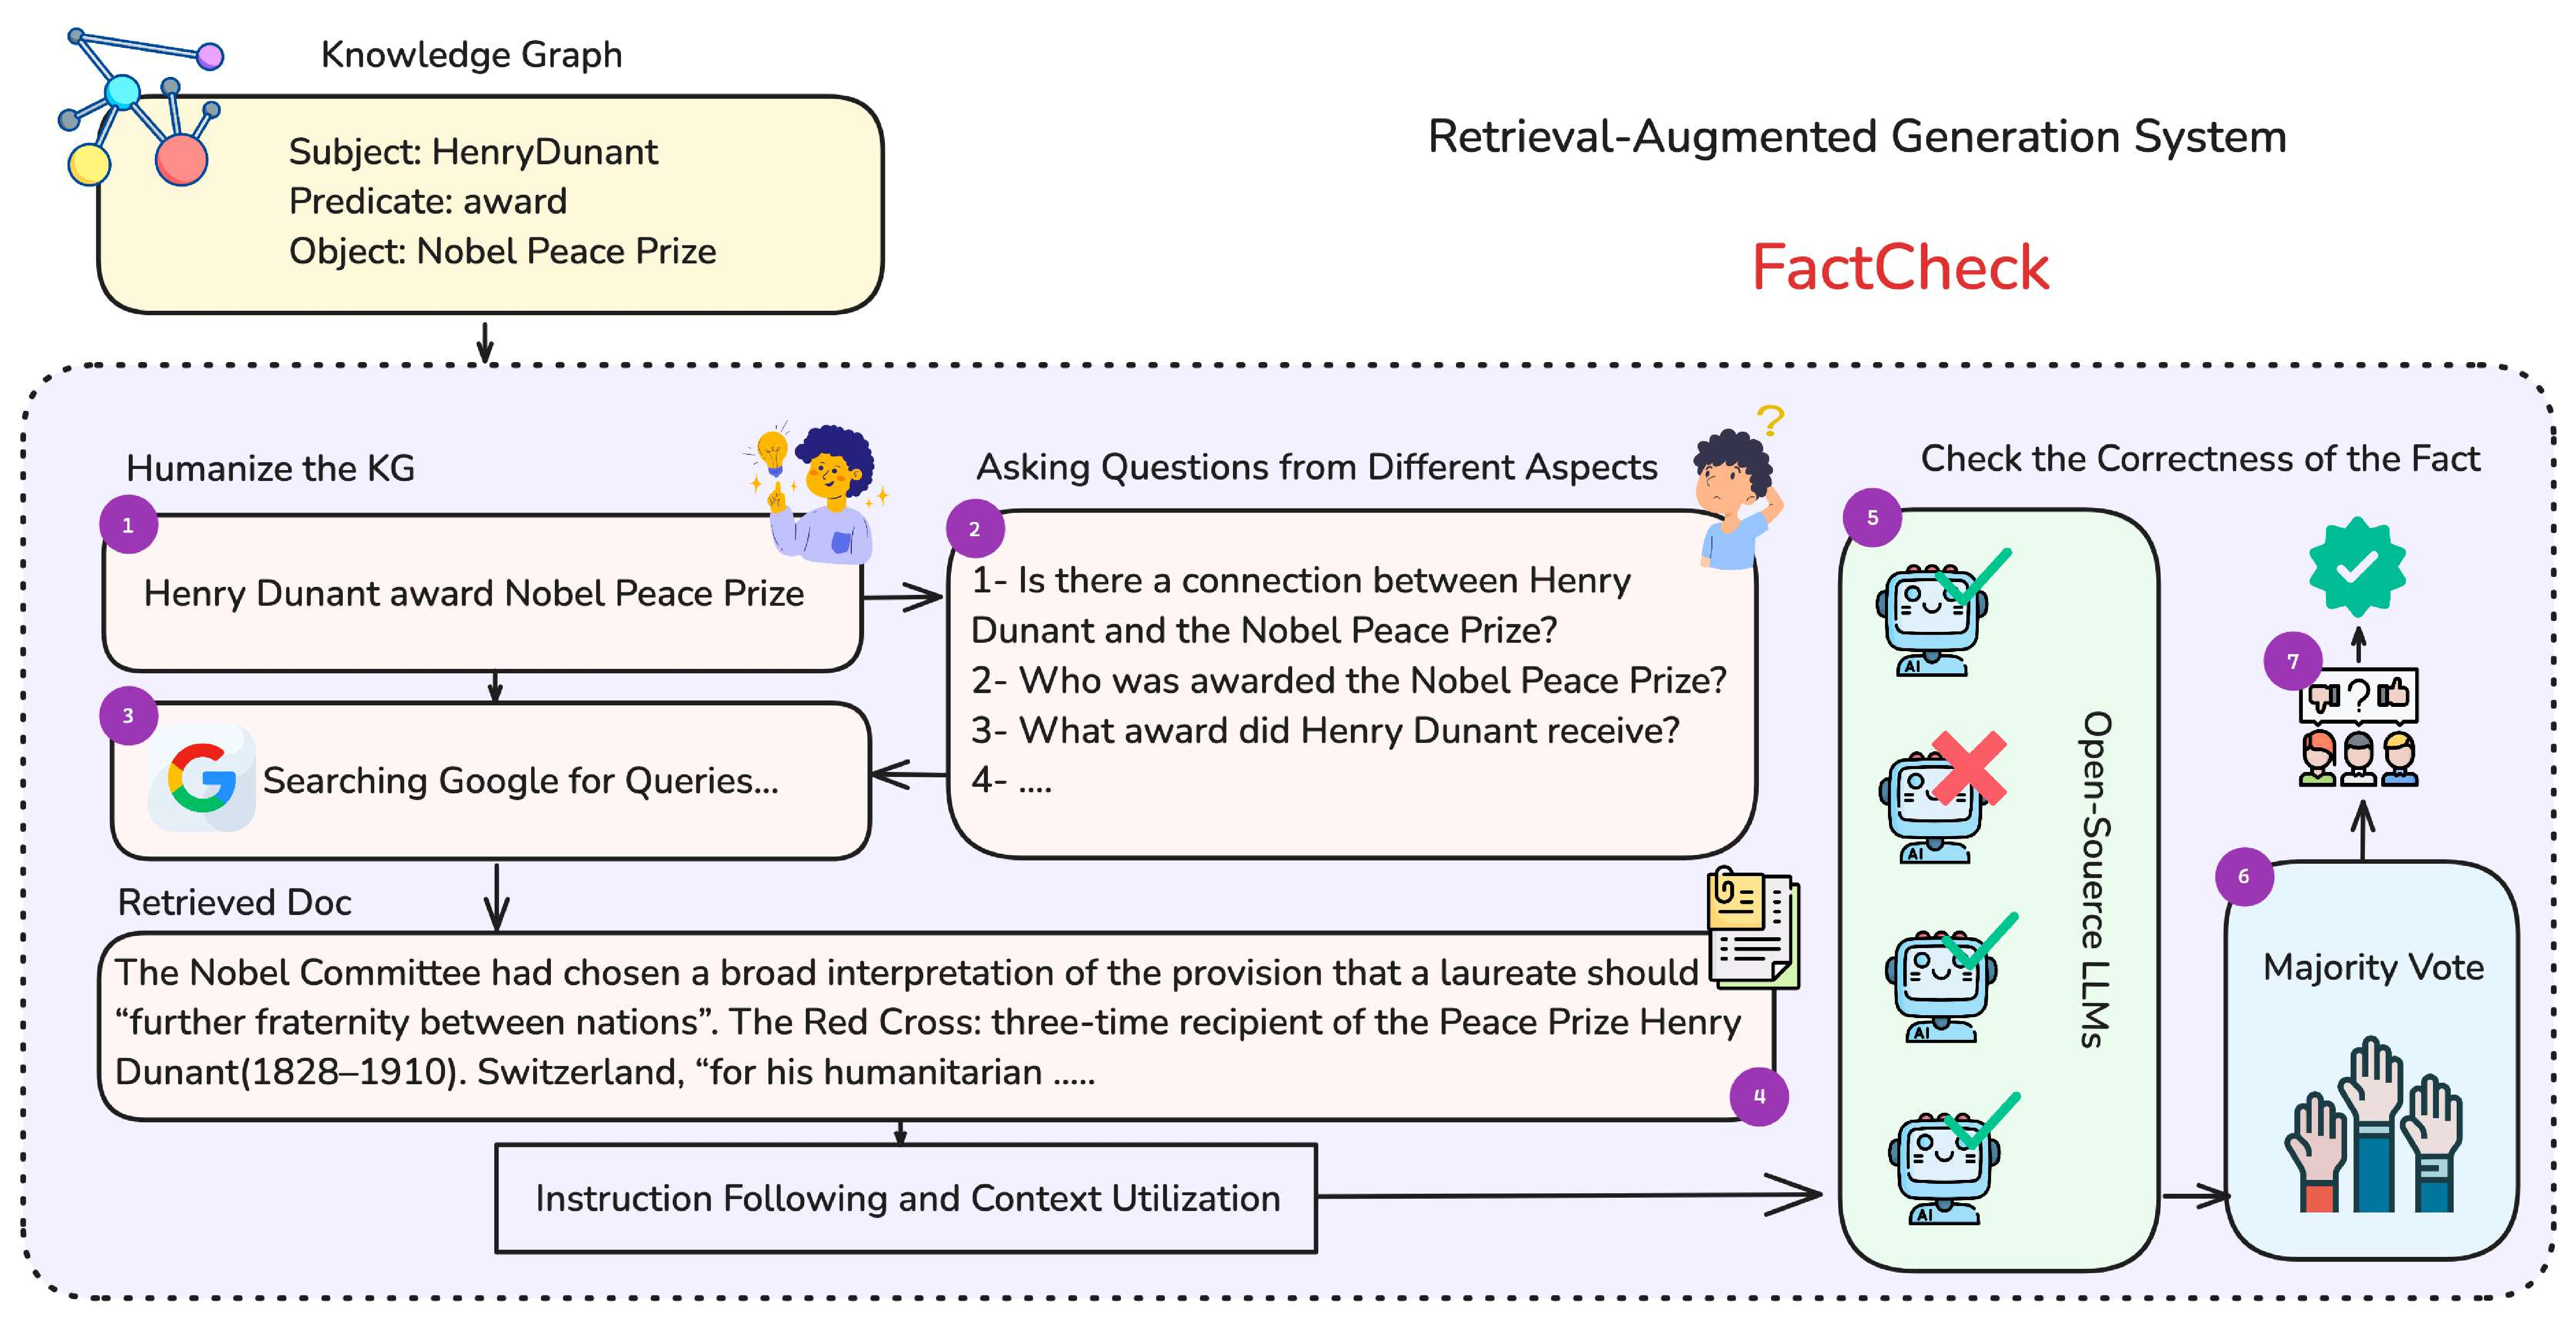
\includegraphics[width=\textwidth]{res/FactCheckOverview}
        \caption{Overview of the FactCheck system for fact verification. The system processes a knowledge graph triple through multiple stages: (1) \ac{KG} humanization, converting structured data into natural language; (2) Generation of aspect-specific questions to probe the fact; (3) Google search retrieval based on generated questions; (4) Analysis of retrieved documents containing relevant information; (5) Deployment of multiple \ac{LLMs} as open-source fact-checkers; (6) Final fact verification through majority voting; and (7) tie-breaker module.}
        \label{fig:factcheck-overview}
    \end{minipage}
\end{figure}
\newpage

The general idea behind the FactCheck system is as follows:
\begin{itemize}
    \item \textbf{\ac{KG} Representation:} We start by representing facts from the \ac{KG} in a format suitable for processing by language models and \ac{IR} systems. This involves converting the subject-predicate-object triples of the \ac{KG} into natural language statements.
    \item \textbf{Query Generation:} For each fact to be verified, we generate multiple queries designed to retrieve relevant information from external sources. These queries are formulated to capture different aspects of the fact and potential supporting or contradicting evidence.
    \item \textbf{\ac{IR}:} We use advanced \ac{IR} techniques to search for relevant documents or passages from a large corpus of trusted sources. This step leverages both traditional search algorithms and dense retrieval methods based on neural networks.
    \item \textbf{Context Processing:} The retrieved information is processed and combined to create a comprehensive context for each fact. This may involve techniques such as text summarization, entity linking, and coreference resolution to create a coherent representation of the relevant information.
    \item \textbf{\ac{LLM} Integration:} We use several \ac{LLMs} at the same time to look at the context that was retrieved and decide if the original fact is true. By putting together the results of several models, we hope to reduce the flaws in each one and make the whole thing more accurate.
    \item \textbf{Fact Verification Decision:} The system makes a final decision on the truthfulness of the fact based on the consensus of the language models and the strength of the supporting or contradicting evidence. This decision is accompanied by the reasoning process and relevant evidence.
\end{itemize}

\section{Contributions}\label{sec:contributions}
This thesis presents several significant contributions to the field of \ac{NLP} and knowledge verification systems.
Our investigation into the capabilities of \acp{LLM} within \ac{RAG} frameworks reveals their considerable potential for fact-verification tasks.
Through experimentation, we have proved that these \acp{LLM} show remarkable aptitude in adapting and contextualizing external knowledge sources which is a crucial capability for reliable information validation in contemporary applications.
By examining \acp{LLM} reasoning patterns and pathways, we provide insights into how these models arrive at verification decisions when confronted with factual claims of varying complexity.
This deeper understanding improves our theoretical grasp of these systems and suggests practical improvements for their implementation in real-world scenarios.

A particularly noteworthy aspect of this work is the assessment of computational efficiency.
Contrary to prevailing assumptions about LLMs that they require substantial computational resources, our findings indicate that effective fact-verification processes can indeed be executed on modestly provisioned local infrastructures.
This finding is important because it makes advanced AI tools more accessible to different research groups, even those with limited resources.

Finally, We conduct error taxonomy that categorizes the failure predication observed during fact-verification task.
Through this analysis, we have identified distinct error categories including context mismatches, relationship errors, role attribution discrepancies, geographic inaccuracies, and more.
This categorization exposes the current limitations of these systems and suggest ways for targeted improvements in subsequent model post-training or fine-tuning.
%
%In general, the key contributions of this work are summarized as follows:
%\begin{enumerate}
%    \item \textbf{Verification of Suitability:} We evaluate the efficacy of \ac{LLMs} in performing fact-verification tasks within \ac{RAG} frameworks, emphasizing their capability to integrate and contextualize external knowledge.
%    \item \textbf{Enhanced Understanding:} We delve into the internal mechanisms of \ac{LLMs} within the \ac{RAG} process, shedding light on their reasoning patterns and decision-making behaviors in fact-validation scenarios.
%    \item \textbf{Resource Efficiency:} We explore the feasibility of executing these procedures locally, aiming to determine whether \ac{LLMs}, often perceived as resource-intensive, can deliver high performance on computationally constrained infrastructures.
%    \item \textbf{Error Taxonomy and Analysis:} We establish a taxonomy of error types encountered in fact-verification scenarios, categorizing them as context mismatches, relationship errors, role attribution discrepancies, geographic inaccuracies, and more. This analysis provides valuable insight into the model's limitations and highlights areas for improvement in future development.
%\end{enumerate}

To evaluate FactCheck, extensive experiments were conducted using four open-source \ac{LLMs} — Gemma2, Qwen2.5, Llama3.1, and Mistral.
These models ranged in size from 7B to 9B parameters, covering various capabilities for dense retrieval, logical reasoning, and interpretability.
Experiments were carried out on 13,530 facts in total.
We used accuracy, F1 scores, computational latency, and resource consumption as core metrics on our evaluations.
Additional ablation studies further validated the efficiency of our system.

\section{Thesis Structure}\label{sec:structure}
The remainder of this thesis is organized as follows:

Chapter~\ref{ch:related_works} provides a comprehensive review of the related works in fact verification, \ac{IR}, and language model applications through \ac{LLMs}.
It situates our work within the broader context of these research areas and highlights the gaps that our system aims to address.
Chapter~\ref{ch:system} presents a detailed description of our proposed FactCheck system for fact verification.
It explains each component of the system, including the rationale behind design choices and implementation details.
Chapter~\ref{ch:empirical-evaluation} describes the experimental setup used to evaluate our system.
This includes details on the datasets used, evaluation metrics, and baseline systems for comparison and offers an in-depth discussion of the results, exploring the implications of our findings and their potential impact on the field of \ac{KG} fact verification.
Chapter~\ref{ch:ablation} Presents a study that investigates the impact of various parameters on the system's overall performance, while also exploring different methodologies for each component to determine the optimal final setting configuration for the system.
% TODO: Check the data here and make sure it's correct, because we see the key components of the system in the previous section.
Finally, chapter~\ref{ch:conclusions} concludes the thesis by summarizing the contributions, discussing limitations of the current approach, and outlining promising directions for future research.

\section{Significance and Potential Applications}\label{sec:significance}
The development of effective fact verification systems for \acp{KG} has far-reaching implications across various domains.
Our system helps ensure accurate information by automatically checking facts, making large knowledge bases more reliable - especially important in today's world, where false information spreads quickly.

It is useful in fields like healthcare, finance, and law, where decisions rely on correct data.
It also helps in education by allowing students to verify information and improve their digital literacy.
The same techniques can be used for content moderation, helping social media and news platforms detect false or misleading content.
In science, the system can check research claims, compare findings, and spot inconsistencies in studies.
By improving fact-checking in \acp{KG}, this thesis supports the goal of building more reliable information systems.